\begin{frame}
\titlepage
\end{frame}

\section{套保案例}

\begin{frame}{下游用铜企业的一年期套保}
假设下游企业在未来一年采购铜，期末按这一年的平均铜价结算。\\
企业买入覆盖同等数量的一年期均价看涨期权，对冲涨价风险。\\[3mm]
执行价为 \textbf{9,000 美元/吨}，今天支付权利金 \textbf{150 美元/吨}。

\medskip
\begin{center}
\setlength{\tabcolsep}{12pt}
\renewcommand{\arraystretch}{1.35}
\begin{tabular}{lrrr}
\toprule
情形 & 年均采购价 & 期权赔付 & 含权利金的净成本 \\
\midrule
年均价高于执行价 & 9,500 & 500 & \textbf{9,150} \\
年均价低于执行价 & 8,700 & 0 & \textbf{8,850} \\
\bottomrule
\end{tabular}
\end{center}
{\fontsize{14}{18}\selectfont 单位均为美元/吨。净成本按名义金额计算，等于采购价减去赔付再加权利金。}

\medskip
记年均价为 \(\bar S\)，执行价为 \(K\)。每吨到期赔付为 \((\bar S-K)^+=\max(\bar S-K,0)\)。

\medskip
已知到期怎么赔，\textbf{今天该为这份保护付多少钱？}
\end{frame}

\section{模型}

\begin{frame}{由布朗运动推导单步价格}
\textbf{1\quad 几何布朗运动}\quad \(S_0\) 初始价，\(W_t\) 标准布朗运动，\(\sigma\) 年化波动率，\(a\) 待定的对数价格漂移。\\
\(T\) 为到期时间（年），\(m\) 为观察次数，\(\Delta t=T/m\)，\(t_j=j\Delta t\)。
\[
 S_t=S_0e^{at+\sigma W_t},
 \qquad W_{t_j}-W_{t_{j-1}}=\sqrt{\Delta t}\,U_j,
 \qquad U_j\overset{\text{独立}}{\sim}\mathcal N(0,1).
\]

\medskip
\textbf{2\quad 确定漂移}\quad \(\mathbb Q\) 为定价概率，\(r\) 为连续复利无风险年利率。\\
对无分红标的，风险中性条件要求单步价格的期望增长倍数为 \(e^{r\Delta t}\)。
\[
 \mathbb E_{\mathbb Q}\!\left[\frac{S_{t_j}}{S_{t_{j-1}}}\right]
 =e^{a\Delta t}\mathbb E_{\mathbb Q}\!\left[e^{\sigma\sqrt{\Delta t}\,U_j}\right]
 =e^{(a+\sigma^2/2)\Delta t}
 =e^{r\Delta t}
 \quad\Longrightarrow\quad a=r-\frac{\sigma^2}{2}.
\]

\textbf{3\quad 递推价格}\quad 令 \(\delta_j=\log(S_{t_j}/S_{t_{j-1}})\) 为第 \(j\) 步的对数收益。
\[
 \delta_j=
 \underbrace{\left(r-\frac{\sigma^2}{2}\right)\Delta t}_{\text{固定部分}}
 +\underbrace{\sigma\sqrt{\Delta t}\,U_j}_{\text{随机部分}},
 \qquad S_{t_j}=S_{t_{j-1}}\,e^{\delta_j}.
\]
\end{frame}

\begin{frame}{从价格路径到期权估值}
按上一页的递推式模拟 \(N\) 条独立路径。\(S_{t_j}^{(i)}\) 为第 \(i\) 条路径的第 \(j\) 个观察价。

\bigskip
\textbf{1\quad 路径内算赔付}\quad 用 \(m\) 个观察价算均价 \(\bar S_i\)，再算折现赔付 \(Y_i\)。
\[
 \bar S_i=\frac1m\sum_{j=1}^m S_{t_j}^{(i)},
 \qquad Y_i=\underbrace{e^{-rT}}_{\text{折现因子}}(\bar S_i-K)^+ .
\]
理论价格为风险中性下折现赔付的期望 \(V_0=\mathbb E_{\mathbb Q}[Y_i]\)。

\bigskip
\textbf{2\quad 跨路径估值}\quad 对 \(Y_i\) 取平均，记 \(s_Y\) 为这些赔付的样本标准差。
\[
 \widehat V_N=\underbrace{\frac1N\sum_{i=1}^N Y_i}_{\text{价格估计}},
 \qquad \underbrace{\widehat{\mathrm{SE}}}_{\text{估计的标准误}}=\frac{s_Y}{\sqrt N}.
\]
固定 \(N\) 时，降低 \(s_Y\) 就能降低标准误。
\end{frame}

\section{算法}

\begin{frame}{几何均价期权为什么有解析价}
\textbf{1\quad 对数均价}\quad \(H\) 为几何均价，\(L=\log H\)。第 \(k\) 次冲击影响从第 \(k\) 次起的 \(m-k+1\) 个观察价。
\[
 L=\frac1m\sum_{j=1}^{m}\log S_{t_j}
   =\mu+\frac{\sigma\sqrt{\Delta t}}{m}\sum_{k=1}^m(m-k+1)\,U_k
   \sim\mathcal N(\mu,v).
\]

\textbf{2\quad 正态参数}\quad \(L\) 服从正态分布，均值为 \(\mu\)，方差为 \(v\)。
\[
 \mu=\log S_0+a\,\frac{T(m+1)}{2m},
 \qquad v=\sigma^2T\frac{(m+1)(2m+1)}{6m^2}.
\]

\textbf{3\quad 解析价}\quad \(L>\log K\) 时有赔付。\(f_L\) 是 \(L\) 的密度，\(\Phi\) 是标准正态的累计概率函数。\\
令 \(d_2=(\mu-\log K)/\sqrt v\)，\(d_1=d_2+\sqrt v\)，则几何期权的今日价格为
\[
 \theta_G=e^{-rT}\int_{\log K}^{\infty}(e^x-K)f_L(x)\,\mathrm dx
 =e^{-rT}\!\left[e^{\mu+v/2}\Phi(d_1)-K\Phi(d_2)\right].
\]
\end{frame}

\begin{frame}{几何支付怎样降低标准误}
同一路径上的算术折现赔付 \(Y_i\) 和几何折现赔付 \(G_i\) 往往同向波动。
\[
 G_i=e^{-rT}(H_i-K)^+,\qquad
 H_i\ \text{为几何均价},\qquad \mathbb E_{\mathbb Q}[G_i]=\theta_G.
\]
用 \(G_i\) 偏离已知均值 \(\theta_G\) 的幅度，估计两种赔付的共同波动。

\medskip
\textbf{1\quad 拟合修正系数}\quad 在 \SlidePilotPaths{} 条独立预备路径上选 \(b\)，使修正后的样本方差最小。
\[
 \widehat\beta
 =\underset{b}{\arg\min}\;\widehat{\operatorname{Var}}\!\bigl(Y-b(G-\theta_G)\bigr)
 =\frac{\widehat{\operatorname{Cov}}(Y,G)}{\widehat{\operatorname{Var}}(G)}.
\]

\textbf{2\quad 修正正式赔付}\quad 固定 \(\widehat\beta\)，在正式路径上扣除估计出的共同波动。
\[
 Z_i=Y_i-\widehat\beta\underbrace{(G_i-\theta_G)}_{\text{期望为零}},
 \qquad \mathbb E_{\mathbb Q}[Z_i\mid\widehat\beta]=V_0.
\]

\textbf{3\quad 估值和标准误}\quad \(s_Z\) 为 \(N\) 条正式路径修正后赔付的样本标准差。
\[
 \widehat V_{\mathrm C}=\frac1N\sum_{i=1}^N Z_i,\qquad
 \widehat{\mathrm{SE}}_{\mathrm C}=\frac{s_Z}{\sqrt N}.
\]
\end{frame}

\begin{frame}{三种模拟方法与实验设置}
\renewcommand{\arraystretch}{1.35}
\begin{tabularx}{\linewidth}{@{}lX@{}}
\toprule
方法 & 怎样计算 \\
\midrule
\textbf{A 全量模拟} & 一次生成并保存全部路径，平均折现支付 \(Y_i\)。 \\
\textbf{B 分块模拟} & 每块最多 20,000 条路径，累积均值和方差所需的统计量。 \\
\textbf{C 分块＋控制变量} & 按 B 的方式分块，在同一路径上算两种支付，再平均修正支付 \(Z_i\)。 \\
\bottomrule
\end{tabularx}

\bigskip
\begin{tabularx}{\linewidth}{@{}l@{\quad}X@{}}
\textbf{基准参数} & \(S_0=K=100\)，\(T=1\) 年，\(m=52\)，观察步长 \(\Delta t=T/m=1/52\) 年。\newline
连续复利无风险年利率 \(r=3\%\)，年化波动率 \(\sigma=20\%\)。 \\[2mm]
\textbf{实验设置} & 正式路径为 1 万、10 万、100 万条，每档用 10 个独立种子。\newline
同一种子共享正式路径，单核计时。C 的耗时包含 5,000 条独立预备路径。 \\
\end{tabularx}
\end{frame}

\section{实验结果}

\begin{frame}{分块省内存，控制变量降低标准误}
\begin{center}
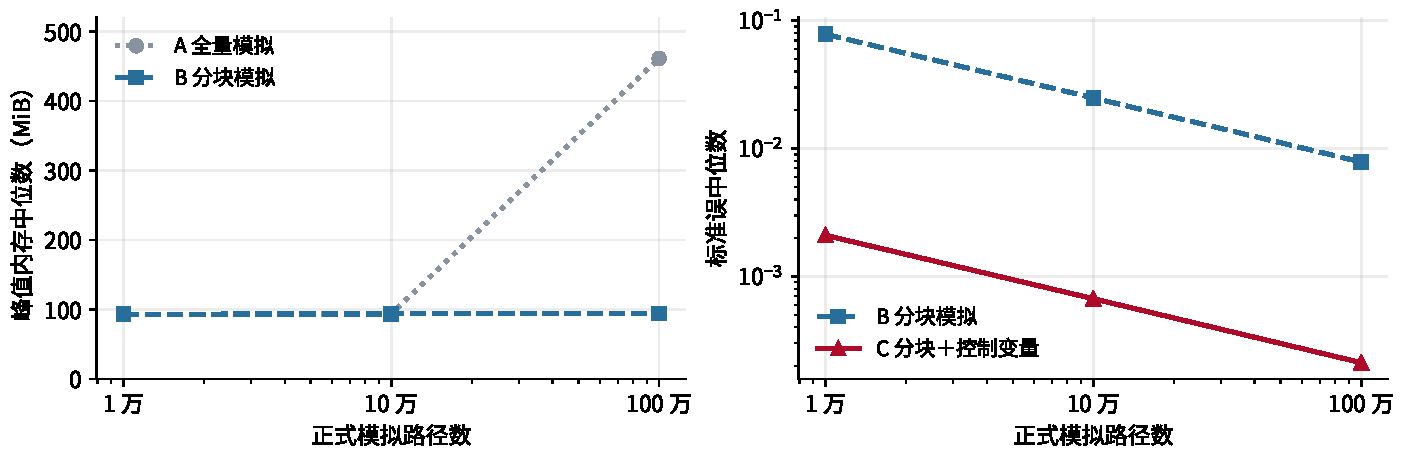
\includegraphics[width=\linewidth,height=88mm,keepaspectratio]{same_paths.pdf}
\end{center}
在 \SlideLargest{} 条正式路径下：
\begin{itemize}
\item \textbf{A 对 B}：峰值内存从 \textbf{\SlideMemoryA{} 降到 \SlideMemoryB{} MiB}，估价一致到显示精度。
\item \textbf{B 对 C}：标准误约为原来的 \textbf{\(1/\SlideSERatio\)}，\\
单次耗时的中位数从 \SlideTimeB{} 秒增至 \SlideTimeC{} 秒。
\end{itemize}
\end{frame}

\begin{frame}{少算路径与并行计算的耗时比较}
\begin{columns}[T,onlytextwidth]
\column{0.60\textwidth}
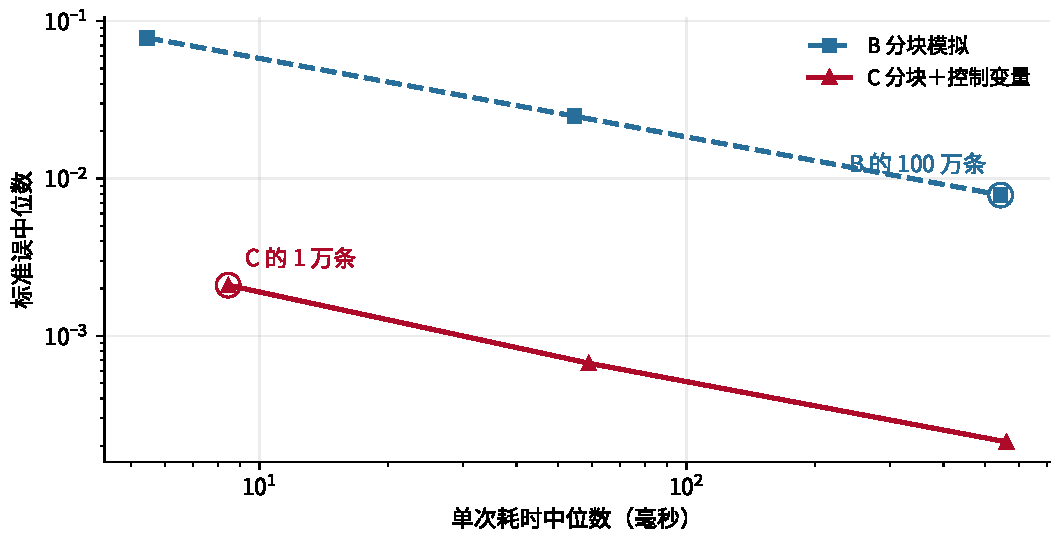
\includegraphics[width=\linewidth]{time_precision.pdf}
\column{0.38\textwidth}
\medskip
\textbf{图中圈出的两组配置}

\medskip
{\fontsize{16}{21}\selectfont\SlideCrossTable}

\bigskip
\textbf{固定 100 万条路径，普通分块}

\smallskip
{\fontsize{16}{21}\selectfont
\begin{tabular}{@{}lr@{}}
\toprule
执行方式 & 耗时中位数（毫秒） \\
\midrule
单核串行 & \ParallelSerialMs \\
6 进程并行 & \ParallelSixMs \\
\bottomrule
\end{tabular}\par}
{\fontsize{16}{21}\selectfont 实测加速比 \textbf{\(\ParallelSpeedup\times\)}，价格与标准误一致。\par}

\end{columns}

\medskip
按种子和重复编号配对，\textbf{B/C 耗时比的中位数为 \SlideCrossRatio}。\\
C 使用 \SlidePilotPaths{} 条独立预备路径，表中耗时已包含这部分计算。
\end{frame}

\section{结论}

\begin{frame}{分块和控制变量各自解决什么}
\begin{itemize}
\item \textbf{分块减少存储。} 用相同的路径估价，峰值内存约降到五分之一。
\item \textbf{控制变量减小估价波动。} 同样的正式路径数下，标准误明显下降。
\item \textbf{并行缩短同一批路径的耗时。} 固定路径数时，6 进程并行取得了实测提速。
\end{itemize}

\bigskip
这些结果来自给定价格模型下的算术均价期权，控制变量的效果取决于两种支付的相关程度。

\bigskip
{\fontsize{13}{17}\selectfont
\textbf{References}\par\smallskip
Kemna, A. G. Z., \& Vorst, A. C. F. (1990). A pricing method for options based on average asset values.\\
\textit{Journal of Banking \& Finance}, 14(1), 113--129.\par\smallskip
Chan, T. F., Golub, G. H., \& LeVeque, R. J. (1983). Algorithms for computing the sample variance: Analysis and recommendations.\\
\textit{The American Statistician}, 37(3), 242--247.\par}
\end{frame}
